\documentclass[12pt]{article}
\usepackage[margin=1.2in]{geometry}
\usepackage[all]{nowidow}
\usepackage[hyperfigures=true, hidelinks, pdfhighlight=/N]{hyperref}
\usepackage[separate-uncertainty=true]{siunitx}
\usepackage{graphicx,amsmath,physics,tabto,float,amssymb,pgfplots,verbatim,tcolorbox}
\usepackage{listings,xcolor,subfig,keyval2e,caption,import}
% \numberwithin{equation}{section}
% \numberwithin{figure}{section}
\definecolor{stringcolor}{HTML}{C792EA}
\definecolor{codeblue}{HTML}{2162DB}
\definecolor{commentcolor}{HTML}{4A6E46}
\lstdefinestyle{appendix}{
    basicstyle=\ttfamily\footnotesize,commentstyle=\color{commentcolor},keywordstyle=\color{codeblue},
    stringstyle=\color{stringcolor},showstringspaces=false,numbers=left,upquote=true,captionpos=t,
    abovecaptionskip=12pt,belowcaptionskip=12pt,language=Python,breaklines=true,frame=single}
\lstdefinestyle{inline}{
    basicstyle=\ttfamily\footnotesize,commentstyle=\color{commentcolor},keywordstyle=\color{codeblue},
    stringstyle=\color{stringcolor},showstringspaces=false,numbers=left,upquote=true,frame=tb,
    captionpos=b,language=Python}
\renewcommand{\lstlistingname}{Appendix}
\pgfplotsset{compat=1.17}

\title{Tutorial 1}
\author{KDSMIL001 \; MAM2046W BP}
\date{\textbf{16 September 2020}}

\begin{document}
    \maketitle
    
    \begin{enumerate}
        \item \textbf{The Laplace Equation on an annulus.}\newline
        We are to solve the following PDE with its boundary conditions:
        \begin{align*}
            \frac{1}{r}\frac{\partial}{\partial r} (r\frac{\partial u}{\partial r})&=-\frac{1}{r^2}\frac{\partial^2 u}{\partial \theta ^2} \\
            u(a,\theta)&=f(\theta)\\
            u(b,\theta)&=g(\theta)\\
            u(r,\pi)&=u(r,-\pi)\\
            u_{\theta}(r,\pi)&=u_{\theta}(r,-\pi)
        \end{align*}
        where $a<r<b$ and $-\pi\leq\theta\leq\pi$. We solve this using separation of variables, 
        starting by splitting $u$ into a product of two functions each dependent on only $r$ or $\theta$:
        \begin{equation*}
            u(r,\theta)=G(r)\Theta(\theta)
        \end{equation*}
        Substituting this back in to our original PDE we get 
        \begin{align*}
            \frac{1}{r}\frac{d}{dr}(r\frac{dG}{dr})\Theta(\theta)&=-\frac{1}{r^2}\frac{d^2\Theta}{d\theta^2}G(r)\\
            \implies \frac{r}{G}\frac{d}{dr}(r\frac{dG}{dr})&=-\frac{1}{\Theta(\theta)}\frac{d^2\Theta}{d\theta^2}
        \end{align*}
        where we have replaced the partial derivatives with full derivatives as $G$ and $\Theta$ are 
        functions of only $r$ or $\theta$. Now we have to choose some constant that both of these ODEs 
        are equal to in order to solve this problem. Since we know how specific solutions behave, we 
        will choose it in such a way that allows the solution of $\Theta$ to be periodic as $\theta$ 
        itself is periodic by nature. So we have 
        \begin{align*}
            \frac{d^2\Theta}{d\theta^2}&=-\lambda\Theta(\theta)\\
            r^2\frac{d^2G}{dr^2}+r\frac{dG}{dr}&=\lambda G
        \end{align*}
        Our BCs will also be affected by this separation:
        \begin{align*}
            \Theta(\pi)&=\Theta(-\pi)\\
            \frac{d\Theta}{d\theta}(\pi)&=\frac{d\Theta}{d\theta}(-\pi)
        \end{align*}
        We will focus on $\Theta$ to begin with:\newline
        For $\lambda>0$ we know the solution to this type of equation:
        \begin{align*}
            \Theta(\theta)&=A\sin(\sqrt{\lambda}\theta)+B\cos(\sqrt{\lambda}\theta)\\
            \implies \frac{d\Theta}{d\theta}&=\sqrt{\lambda}(A\cos(\sqrt{\lambda}\theta)-B\sin(\sqrt{\lambda}\theta))
        \end{align*}
        Applying our BCs we have 
        \begin{align*}
            A\sin(\sqrt{\lambda}\pi)+B\cos(\sqrt{\lambda}\pi)&=A\sin(-\sqrt{\lambda}\pi)+B\cos(-\sqrt{\lambda}\pi)\\
            &=-A\sin(\sqrt{\lambda}\pi)+B\cos(\sqrt{\lambda}\pi)\\
            \implies 2A\sin(\sqrt{\lambda}\pi)&=0\\
            \implies A\sin(\sqrt{\lambda}\pi)&=0\\
            \sqrt{\lambda}(A\cos(\sqrt{\lambda}\pi)-B\sin(\sqrt{\lambda}\pi))&=\sqrt{\lambda}(A\cos(-\sqrt{\lambda}\pi)-B\sin(-\sqrt{\lambda}\pi))\\
            \implies A\cos(\sqrt{\lambda}\pi)-B\sin(\sqrt{\lambda}\pi)&=A\cos(\sqrt{\lambda}\pi)+B\sin(\sqrt{\lambda}\pi)\\
            \implies 2B\sin(\sqrt{\lambda}\pi)&=0\\
            \implies B\sin(\sqrt{\lambda}\pi)&=0
        \end{align*}
        We can't have $A=B=0$ as that's the trivial solution, so it must be that 
        \begin{align*}
            \sqrt{\lambda}\pi&=n\pi\;;\;n\in\mathbb{Z}\\
            \implies \lambda&=n^2\;;\;n\in\mathbb{Z}
        \end{align*}
        So our solution is
        \begin{equation*}
            \Theta(\theta)=A\sin(n\theta)+B\cos(n\theta)\;;\;n\in\mathbb{Z}
        \end{equation*}
        We also know from doing this before that $\lambda<0$ has no eigenvalues for this problem, and 
        $\lambda=0$ has one eigenfunction and that is $\Theta(\theta)=C\;;\; C\in\mathbb{R}$.\newline
        Now we look at $G$. We know $\lambda=n^2$, so we have
        \begin{equation*}
            r^2\frac{d^2G}{dr^2}+r\frac{dG}{dr}-n^2 G=0
        \end{equation*}
        which we recognise as being an Euler ODE, which we solve with the ansatz $G(r)=r^s,\;r>0$. We 
        then get the characteristic equation of 
        \begin{equation*}
            s(s-1)+s-n^2=0
        \end{equation*}
        which has the solution $s=\pm n$. Now we split the problem into two cases. \newline
        Firstly we have $n\neq0$ which has the general solution
        \begin{equation*}
            G(r)=Dr^n + Er^{-n}
        \end{equation*}
        And then $n=0$, which has general solution 
        \begin{equation*}
            G(r)=F+H\log(r)
        \end{equation*}
        By the superposition principle we can find the general solution regardless of the value of $n$ 
        by summing these solutions, so we finally have 
        \begin{equation*}
            G(r)=Dr^n + Er^{-n} + F+H\log(r)
        \end{equation*}
        and so we have 
        \begin{equation*}
            u(r,\theta)=G(r)\Theta(\theta)=(Dr^n + Er^{-n} + F+H\log(r))(A\sin(n\theta)+B\cos(n\theta))\;;\;n\in\mathbb{Z}
        \end{equation*}
        And now we can write it in its infinite sum form, the most general solution:
        \begin{equation*}
            u(r,\theta)=\sum_{n=1}^{\infty}(D_nr^n + E_nr^{-n} + F_n+H_n\ln(r))(A_n\sin(n\theta)+B_n\cos(n\theta))
        \end{equation*}
        And at this point I'm lost..

        \item \textbf{Chemical Diffusion through a thin layer described by}
        \begin{equation*}
            \frac{\partial C}{\partial t}=\frac{\partial^2 C}{\partial x^2}-he^{-x}
        \end{equation*}
        This has BCs and ICs
        \begin{align*}
            C(0,t)&=10\\
            C(L,t)&=20\;,\;t>0\\
            C(x,0)&=x\;\text{for}\; 0<x\leq\frac{L}{2}\\
            C(x,0)&=0\;\text{for}\; \frac{L}{2}<x<L
        \end{align*}

        \begin{enumerate}
            \item To solve this PDE, we cannot use separation of variables as that depends on having 
            a homogeneous PDE as well as homogeneous BCs. What we can start with, however, is finding 
            the equilibrium solution, that is the solution independent of $t$, which we will call $C_E$.
            This solution must satisfy the following conditions.
            \begin{align*}
                \frac{\partial C_E}{\partial t}&=\frac{\partial^2 C_E}{\partial x^2}-he^{-x}\\
                \implies C_E''&=he^{-x}\\
                C_E(0)&=10\\
                C_E(L)&=20
            \end{align*}
            The partial derivatives become full derivatives as $C_E$ is a function of only $x$.
            To solve for $C_E$ we do 
            \begin{align*}
                C_E''&=he^{-x}\\
                \implies C_E'&=\int_0^z he^{-s} ds +A\\
                \implies C_E&=\int_0^x \int_0^z he^{-s} ds dz +Ax+B\\
                &=h\int_0^x [-e^{-s}]_0^z dz+ Ax+B\\
                &=h\int_0^x (-e^{-z}-(-1))dz+Ax+B\\
                &=h[e^{-z}+z]_0^x +Ax+B\\
                C_E&=h(e^{-x}+x-1)+Ax+B
            \end{align*}
            Now we can impose our BCs:
            \begin{align*}
                C_E(0)=10&=he^0+h(0)-h+A(0)+B\\
                &=B\\
                C_E(L)=20&=he^{-L}+hL-h+AL+10\\
                \implies A&=\frac{1}{L}(10-h(e^{-L}+L-1))\\
                \implies C_E(x)&=h(e^{-x}+x-1)+\frac{x}{L}(10-h(e^{-L}+L-1))+10
            \end{align*}
            This is the equilibrium solution to our PDE but in order to get a complete solution that 
            works for any $t$ we need to consider a small perturbation away from the equilibrium, what 
            we will call $v(x,t)=C(x,t)-C_E(x)$. Substituting this back into our original PDE we get 
            \begin{align*}
                \frac{\partial C}{\partial t}&=\frac{\partial^2 C}{\partial x^2}-he^{-x}\\
                \implies \frac{\partial v}{\partial t}&=\frac{\partial^2 C_E}{\partial x^2}+\frac{\partial^2 v}{\partial x^2}-he^{-x}\\
                \implies \dot{v}&=C_E''+v''-he^{-x}\\
                \implies \dot{v}&=he^{-x}+v''-he^{-x}\\
                \implies \dot{v}&=v''
            \end{align*}
            which is the homogeneous heat equation! We know how to solve these. Better yet, we can examine 
            the BCs:
            \begin{align*}
                C(0,t)=10&=C_E(0)+v(0,t)\\
                &=10+v(0,t)\\
                \implies v(0,t)&=0\\
                C(L,t)=20&=C_E(L)+v(L,t)\\
                &=20+v(L,t)\\
                \implies v(L,t)&=0
            \end{align*}
            So our BCs are homogeneous too! How wonderful! We know exactly how to solve these using separation 
            of variables, which will result in 
            \begin{equation*}
                v(x,t)=\sum_{n=1}^\infty C_n\sin(\frac{n\pi x}{L})e^{-\frac{n^2\pi^2kt}{L^2}}
            \end{equation*}
            The ICs for this problem give us two cases:\newline
            For $0<x\leq\frac{L}{2}$
            \begin{align*}
                C(x,0)=x&=C_E(x)+v(x,0)\\
                \implies v(x,0)&=x-C_E(x)\\
                \implies x-C_E(x)&=\sum_{n=1}^\infty C_n\sin(\frac{n\pi x}{L})\\
                \implies C_n&=\frac{4}{L} \Bigl< x-C_E(x) \Big| \sin(\frac{n\pi x}{L}) \Bigr>\\
                &= \frac{4}{L}\int_0^{\frac{L}{2}} (x-(h(e^{-x}+x-1)+\frac{x}{L}(10-h(e^{-L}+L-1))+10))(\sin(\frac{n\pi x}{L}))dx
            \end{align*}
            And now $\frac{L}{2}<x<L$ gives
            \begin{align*}
                C(x,0)=o&=C_E(x)+v(x,0)\\
                \implies v(x,0)&=-C_E(x)\\
                \implies -C_E(x)&=\sum_{n=1}^\infty C_n\sin(\frac{n\pi x}{L})\\
                \implies C_n&=\frac{4}{L}\Bigl<-C_E(x) \Big| \sin(\frac{n\pi x}{L})\Bigr>\\
                &= \frac{4}{L} \int_{\frac{L}{2}}^L (h(e^{-x}+x-1)+\frac{x}{L}(10-h(e^{-L}+L-1))+10)(\sin(\frac{n\pi x}{L}))dx
            \end{align*}

            And so we finally have a solution:
            \begin{equation*}
                C(x,t)=h(e^{-x}+x-1)+\frac{x}{L}(10-h(e^{-L}+L-1))+10 + \sum_{n=1}^\infty C_n\sin(\frac{n\pi x}{L})e^{-\frac{n^2\pi^2kt}{L^2}}
            \end{equation*}
            with $C_n$ given above depending on the region.

            \item As $t\rightarrow\infty$, $e^{-t}\rightarrow 0$, meaning the entire $v(x,t)$ solution goes to
            0, leaving $C(x,t)$ to be made up only of the equilibrium solution.

            \item \textbf{Even extension of the initial condition}
            \begin{figure}[H]
                \begin{center}
                   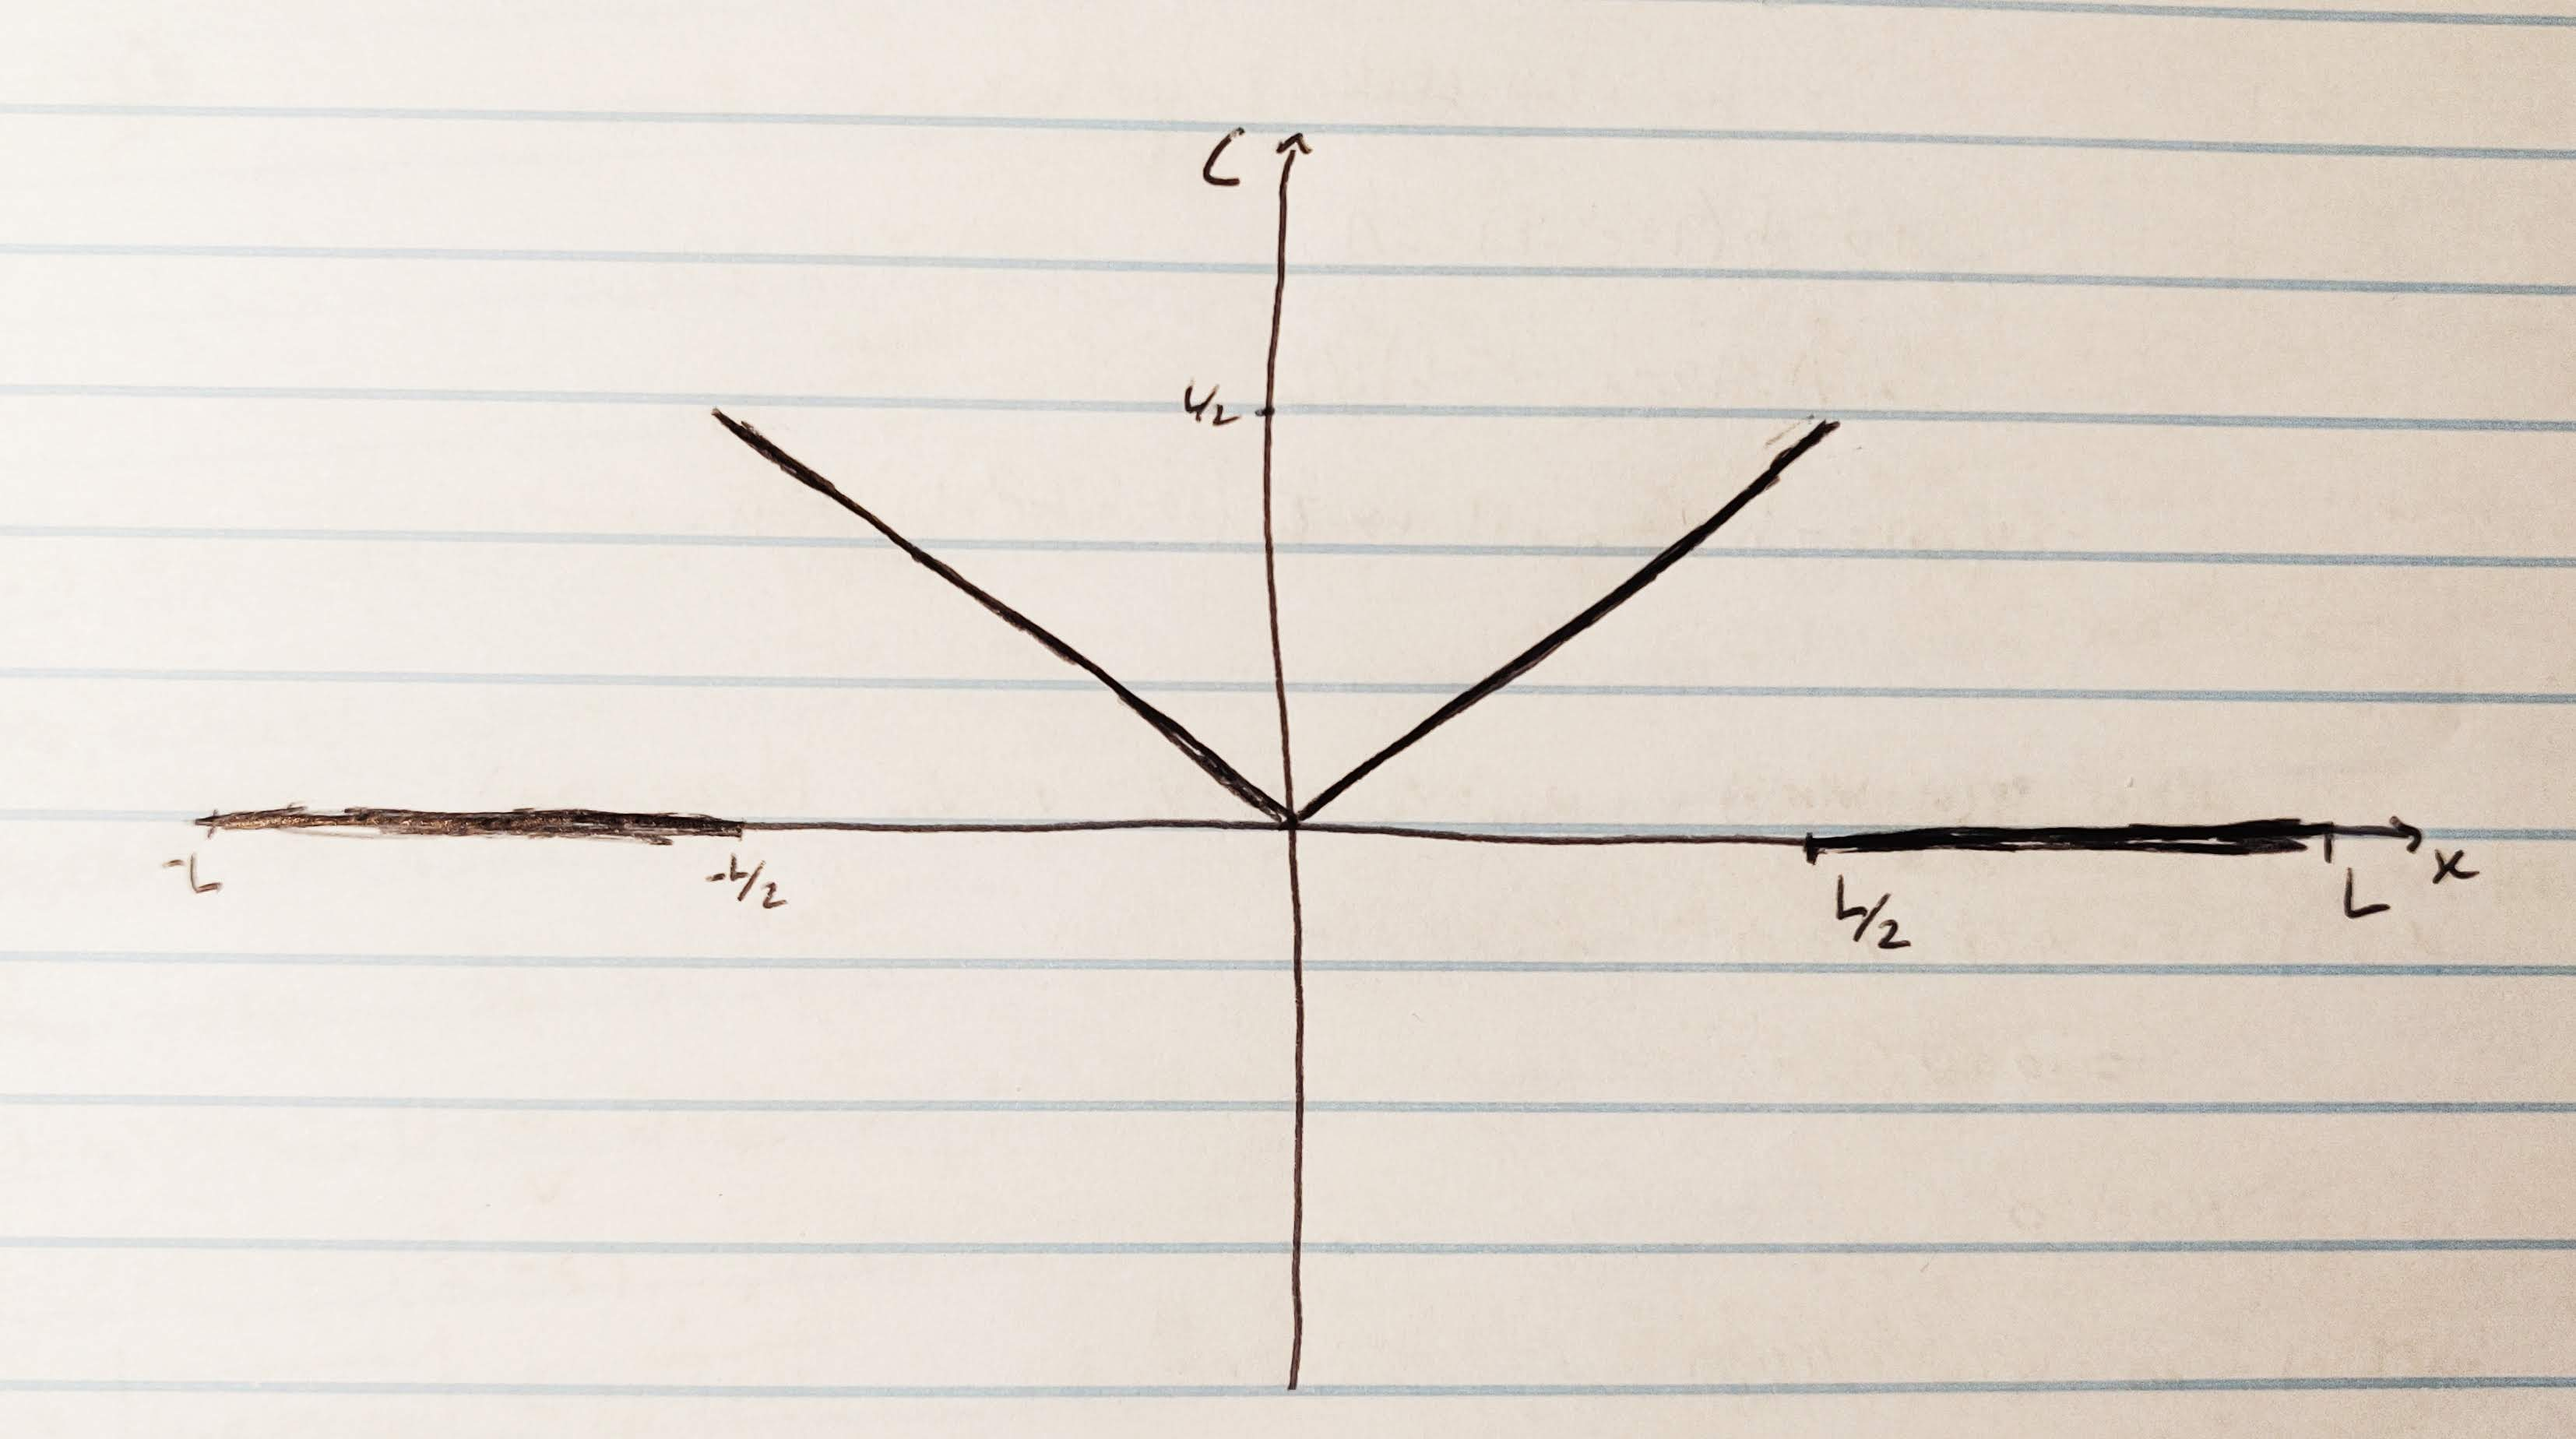
\includegraphics[width=.65\textwidth]{EvenExtension.jpg}
                   \caption{The even extension of the initial condition $C(x,0)=x\;\text{for}\; 0<x\leq\frac{L}{2},\;C(x,0)=0\;\text{for}\; \frac{L}{2}<x<L$}
                   \label{fig:EvenExtension}
                \end{center}
            \end{figure}

            \item \textbf{Odd extension of the initial condition}
            \begin{figure}[H]
                \begin{center}
                   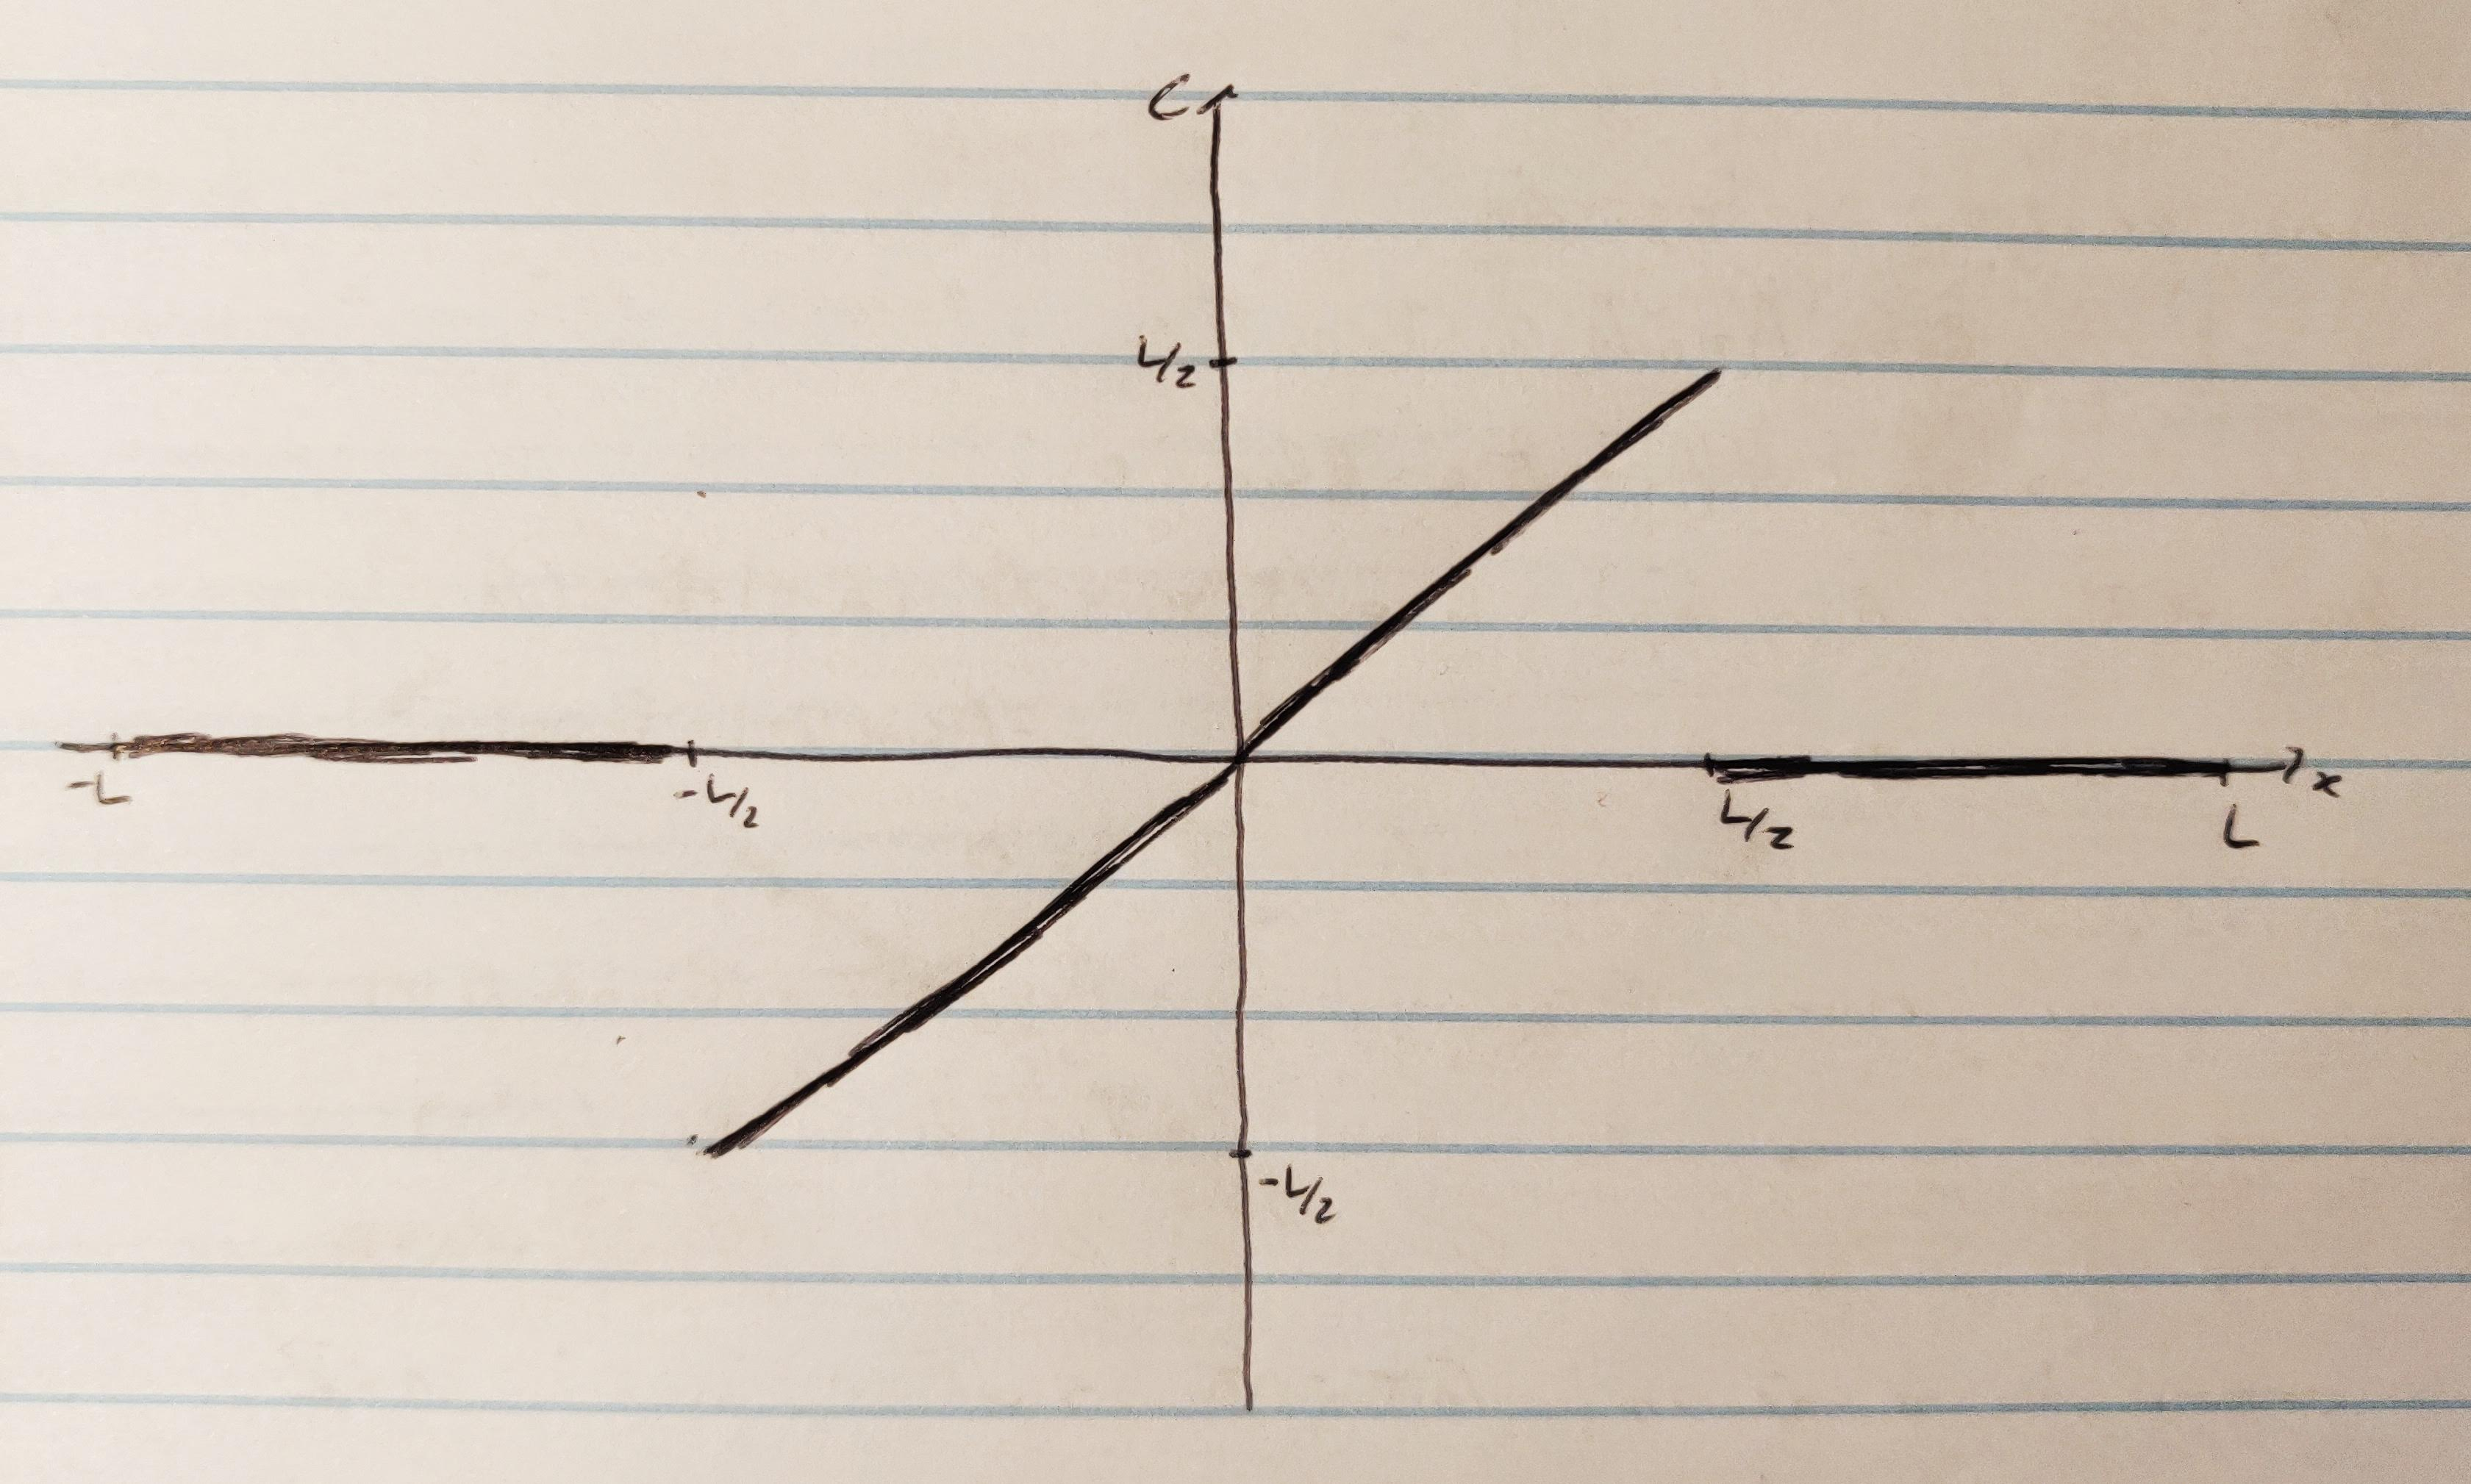
\includegraphics[width=.65\textwidth]{OddExtension.jpg}
                   \caption{The odd extension of the initial condition $C(x,0)=x\;\text{for}\; 0<x\leq\frac{L}{2},\;C(x,0)=0\;\text{for}\; \frac{L}{2}<x<L$}
                   \label{fig:OddExtension}
                \end{center}
            \end{figure}            
        
            \item \textbf{Fourier series of the odd extension of the initial condition}
            \begin{figure}[H]
                \begin{center}
                       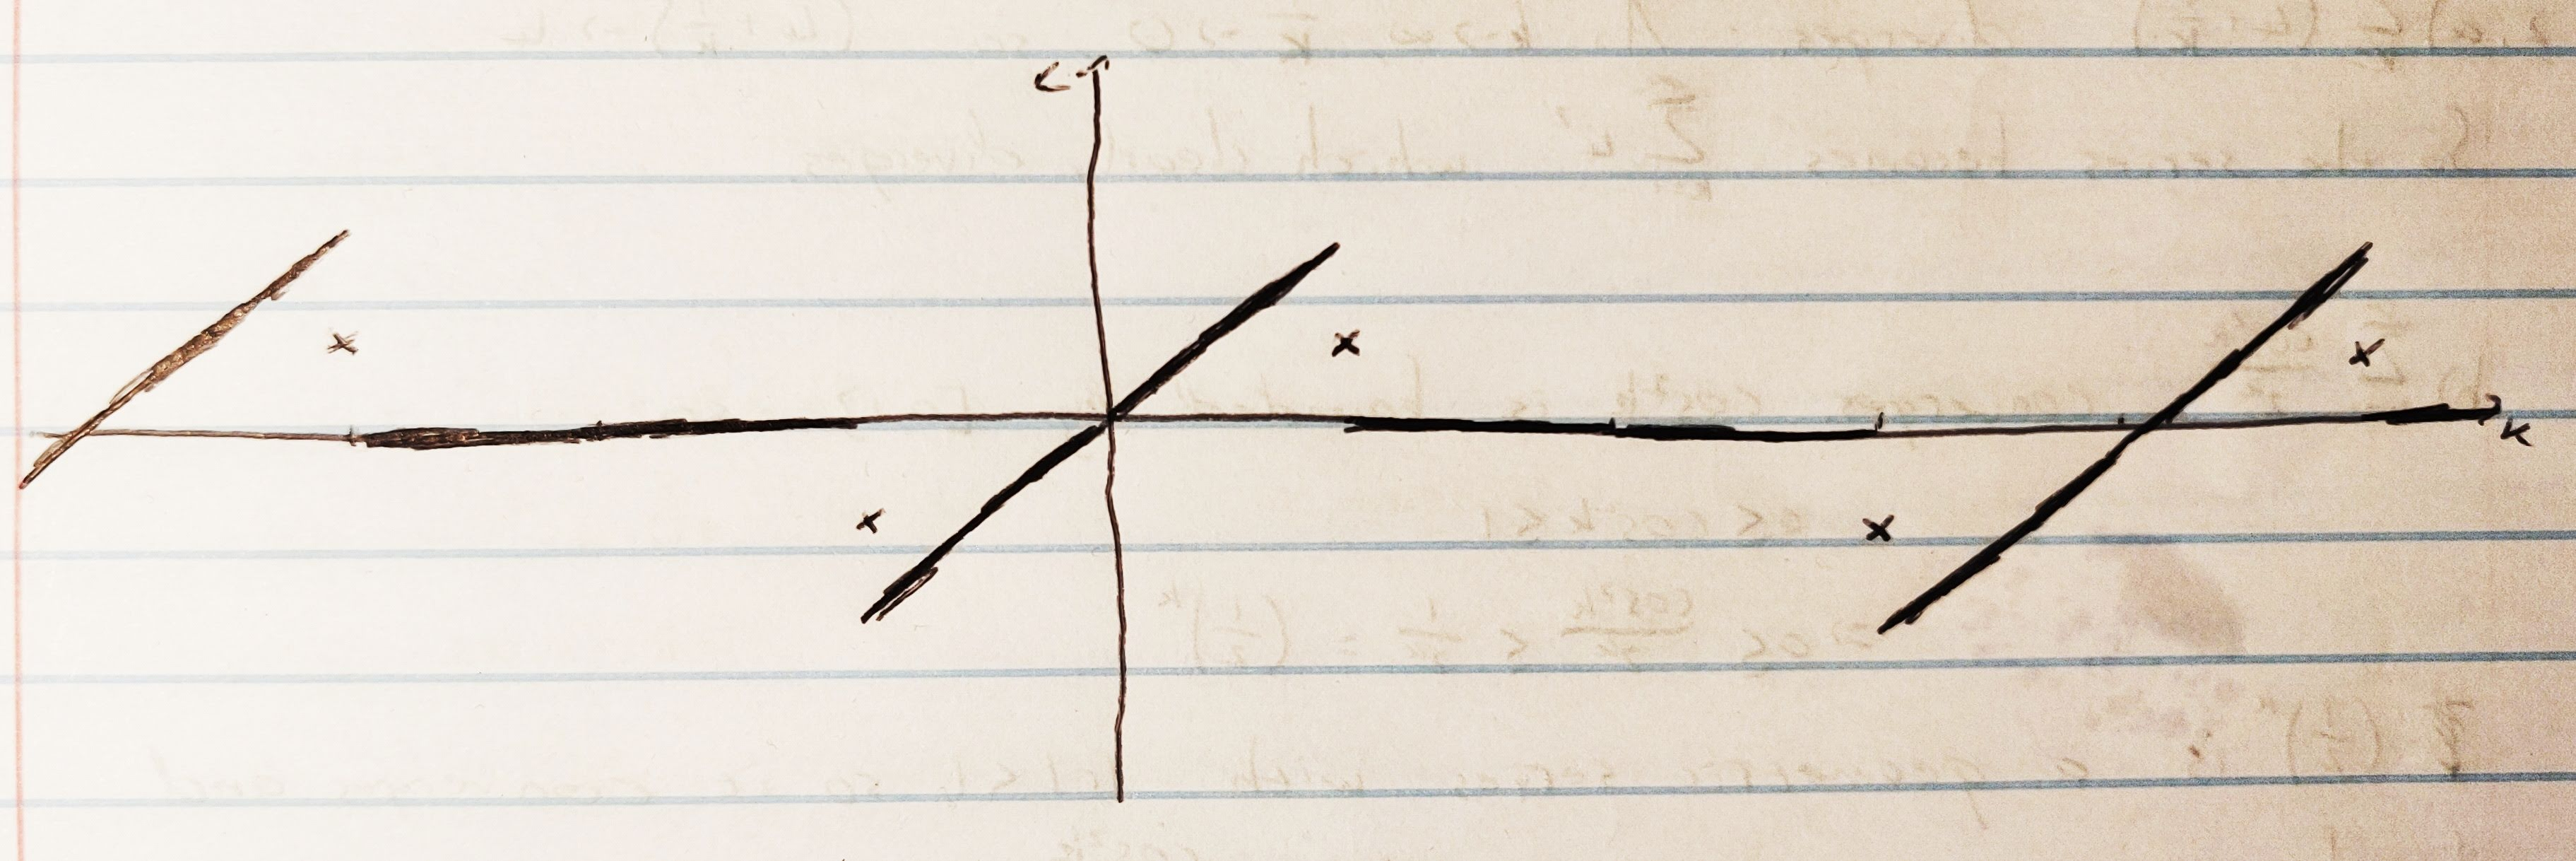
\includegraphics[width=.65\textwidth]{OddFourier.jpg}
                       \caption{The fourier series of the odd extension of the initial condition $C(x,0)=x\;\text{for}\; 0<x\leq\frac{L}{2},\;C(x,0)=0\;\text{for}\; \frac{L}{2}<x<L$}
                       \label{fig:OddFourier}
                    \end{center}
                \end{figure}
                
        \end{enumerate}

        \item \textbf{Laplace BVP on a rectangle}\newline
        We are to solve the following BVP:
        \begin{align*}
            \frac{\partial^2 V}{\partial x^2}+\frac{\partial ^2 V}{\partial y^2}&=0\\
            V_x(0,y)=V_x(\pi,y)&=0\;,\;0\leq y\leq1\\
            V(x,0)&=\cos(x)-\cos(3x)\;,\;0\leq x\leq\pi\\
            V(x,1)&=\cos(2x)\;,\;0\leq x\leq\pi
        \end{align*}
        for $0<x<\pi$ and $0<y<1$. We will solve this using separation of variables but not quite in the 
        usual way. Since we have more than one non-homogeneous BC we are going to have to solve this twice, 
        once for each non-homogeneous BC, and sum the two results to get a general solution.\newline
        To begin we say 
        \begin{align*}
            V(x,y)&=X(x)Y(y)\\
            \implies \frac{1}{X}\frac{d^2 X}{dx^2}&=-\frac{1}{Y}\frac{d^2 Y}{dy^2}
        \end{align*}
        Now we can set them both to a constant to solve them individually. We will do this in such a way 
        that leaves $X$ with oscillatory solutions:
        \begin{align*}
            \frac{d^2 X}{dx^2}&=-\lambda X\\
            \frac{d^2 Y}{dy^2}&=\lambda Y
        \end{align*}
        Starting with $X$, we know the solution to this, which gives us
        \begin{align*}
            X(x)&=A\sin(\sqrt{\lambda}x)+B\cos(\sqrt{\lambda}x)\\
            X'(x)&=\sqrt{\lambda}(A\cos(\sqrt{\lambda}x)-B\sin(\sqrt{\lambda}x))
        \end{align*}
        and our BCs become $X'(0)=X'(\pi)=0$ which give us
        \begin{align*}
            X'(0)=0&=A\cos(0)-B\sin(0)\\
            &=A\\
            X'(\pi)=0&=-B\sin(\sqrt{\lambda}\pi)
        \end{align*}
        But we can't have that $A=B=0$ as that's trivial, so it must be that 
        \begin{align*}
            \sqrt{\lambda}\pi&=n\pi\;,\;n\geq 0\\
            \implies \lambda&=n^2\;,\;n\geq 0
        \end{align*}
        So we have a final solution and infinite sum solution of 
        \begin{align*}
            X(x)&=B\cos(nx)\;,\;n\geq 0\\
            X(x)&=\sum_{n=0}^\infty B_n\cos(nx)
        \end{align*}
        Now we can look at $Y$. Again we have a standard ODE that we know how to solve, especially 
        since we know the value of $\lambda$:
        \begin{equation*}
            Y(y)=C\sinh(ny)+D\cosh(ny)\;,\;n\geq 0
        \end{equation*}
        But now we deviate from the usual process. We will split this problem into two cases. Firstly 
        we look at the case where $Y(0)=0$, then where $Y(1)=0$.\newline
        \textbf{Case 1:}$Y(0)=0,\;Y(1)=\cos(2x)$ This BC lets us simplify some things
        \begin{align*}
            Y(0)=0&=C\sinh(0)+D\cosh(0)\\
            &=D\\
            \implies Y(y)&=C\sinh(ny)\;,\;n\geq 0
        \end{align*}
        And then we have the infinite sum solution
        \begin{equation*}
            Y(y)=\sum_{n=0}^\infty C_n \sinh(ny)
        \end{equation*}
        At this point we're going to combine $X$ and $Y$ back into $V$ and get 
        \begin{equation*}
            V_1(x,y)=\sum_{n=0}^\infty A_{1,n}\cos(nx)\sinh(ny)
        \end{equation*}
        Now we can impose the last BC, which acts like an IC in this case:
        \begin{align*}
            V_1(x,1)=\cos(2x)&=\sum_{n=1}^\infty A_{1,n}\cos(nx)\sinh(n)\\
            \implies A_{1,n}&=\frac{2}{\pi\sinh(n)}\Bigl< \cos(2x) \Big| \cos(nx) \Bigr>
        \end{align*}
        This inner product evaluates to 0 for $n\neq2$ and to $\frac{\pi}{2}$ for $n=2$. So $A_{1,n}$ is 
        only non-zero for $n=2$. So we have 
        \begin{equation*}
            V_1(x,y)=\frac{1}{\sinh(2)}\cos(2x)\sinh(2y)
        \end{equation*}
        \newline
        \textbf{Case 2:}$Y(0)=\cos(x)-\cos(3x),\;Y(1)=0$ Now we do the same as above:
        \begin{align*}
            Y(1)=0&=C\sinh(n)+D\cosh(n)
        \end{align*}
        This doesn't help us. However, we can notice that another solution to the $Y$ ODE is 
        \begin{equation*}
            Y(y)=C\sinh(n(y-1))+D\cosh(n(y-1))
        \end{equation*}
        Using this and applying our BC, we get 
        \begin{align*}
            Y(1)=0&=C\sinh(0)+D\cosh(0)\\
            &=D\\
            \implies Y(y)&=C\sinh(n(y-1))
        \end{align*}
        So we have 
        \begin{equation*}
            V_2(x,y)=\sum_{n=0}^\infty A_{2,n}\cos(nx)\sinh(n(y-1))
        \end{equation*}
        Applying our IC we have 
        \begin{align*}
            V_2(x,0)=\cos(x)-\cos(3x)&=\sum_{n=0}^\infty A_{2,n}\cos(nx)\sinh(n(-1))\\
            &=-\sum_{n=0}^\infty A_{2,n}\cos(nx)\sinh(n)\\
            \implies A_{2,n}&=\frac{-2}{\pi\sinh(n)} \Bigl< \cos(x)-\cos(3x) \Big| \cos(nx) \Bigr>\\
            &=\frac{-2}{\pi\sinh(n)} \left[ \int_0^\pi \cos(x)\cos(nx) dx - \int_0^\pi \cos(3x)\cos(nx) \right]
        \end{align*}
        As in Case 1 we have that the constant goes to 0 everywhere but certain values of $n$. Leaving us with 
        \begin{align*}
            A_{2,1}&=\frac{-2}{\pi\sinh(1)} \frac{\pi}{2}\\
            &= \frac{-1}{\sinh(1)}\\
            A_{2,3}&=\frac{2}{\pi\sinh(n)} \frac{\pi}{2}\\
            &= \frac{1}{\sinh(3)}
        \end{align*}
        So we have two solutions for this case:
        \begin{align*}
            V_{2,1}&=\frac{-1}{\sinh(1)}\cos(x)\sinh(y-1)\\
            V_{2,3}&=\frac{1}{\sinh(3)}\cos(3x)\sinh(3y-3)
        \end{align*}
        \newline
        \newline
        Finally, we can combine all of our cases for a general solution:
        \begin{equation*}
            V(x,y)=\frac{1}{\sinh(2)}\cos(2x)\sinh(2y)+\frac{-1}{\sinh(1)}\cos(x)\sinh(y-1)+\frac{1}{\sinh(3)}\cos(3x)\sinh(3y-3)
        \end{equation*}
    \end{enumerate}

\end{document}